\documentclass[tikz,border=3mm]{standalone}
\usepackage[T1]{fontenc}
\usepackage[utf8]{inputenc}
\usepackage{mathptmx}
\usetikzlibrary{arrows.meta,positioning,calc,shapes.geometric}
\definecolor{ink}{HTML}{202A33}
\definecolor{blue}{HTML}{2D7F9D}
\definecolor{orange}{HTML}{C97728}
\definecolor{light}{HTML}{B0C0D0}
\definecolor{soft}{HTML}{F3F5F7}
\begin{document}
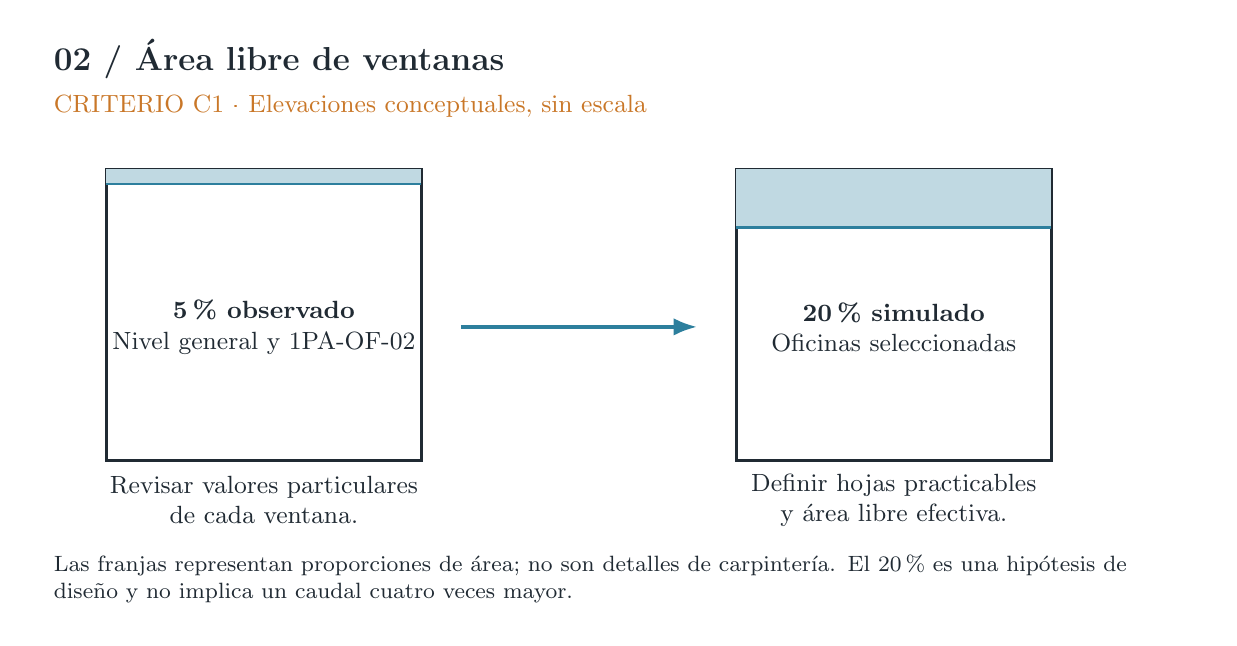
\begin{tikzpicture}[x=1cm,y=1cm,>=Latex,line width=.9pt,every node/.style={font=\rmfamily\small,text=ink},note/.style={align=left,text width=4.1cm,anchor=west},flow/.style={->,blue,line width=1.2pt}]
\path[use as bounding box] (0,0) rectangle (15,7.5);


\node[anchor=west,font=\rmfamily\bfseries\large] at (.2,7.1) {02 / Área libre de ventanas};
\node[anchor=west,text=orange] at (.2,6.5) {CRITERIO C1 · Elevaciones conceptuales, sin escala};
\draw[ink] (1,2) rectangle (5,5.7);
\fill[blue!30] (1,5.515) rectangle (5,5.7);
\draw[blue] (1,5.515)--(5,5.515);
\draw[ink] (9,2) rectangle (13,5.7);
\fill[blue!30] (9,4.96) rectangle (13,5.7);
\draw[blue] (9,4.96)--(13,4.96);
\node[align=center] at (3,3.7) {\textbf{5\,\% observado}\\Nivel general y 1PA-OF-02};
\node[align=center] at (11,3.7) {\textbf{20\,\% simulado}\\Oficinas seleccionadas};
\draw[flow] (5.5,3.7)--(8.5,3.7);
\node[align=center,text width=5cm] at (3,1.5) {Revisar valores particulares\\de cada ventana.};
\node[align=center,text width=5cm] at (11,1.5) {Definir hojas practicables\\y área libre efectiva.};
\node[anchor=west,text width=14cm,align=left,font=\rmfamily\footnotesize] at (.2,.5) {Las franjas representan proporciones de área; no son detalles de carpintería. El 20\,\% es una hipótesis de diseño y no implica un caudal cuatro veces mayor.};

\end{tikzpicture}
\end{document}
